% #############################################################################
% This is Chapter 4
% !TEX root = ../main.tex
% #############################################################################
% Change the Name of the Chapter i the following line
\fancychapter{Experimental Work \& Results}
\cleardoublepage
% The following line allows to ref this chapter
\label{chap:results}

So far, we have introduced the theme to be developed in this thesis in Chapter \ref{chap:intro}, we have presented some studies developed in this area in Chapter \ref{chap:background}, and we have presented the specific case studied approached in this thesis during Chapter \ref{chap:architecture}. In this chapter, we present the experimental procedure put into practice, and the results obtained.



\section{Initial considerations}

Before diving into the details of the experimental work, it is necessary to establish a baseline for the results obtained. Without establishing the basis it is quite difficult to know what kind of values to expect during the development of the predictive models. In order to establish a comparative basis, a baseline model was developed which can be called the Naive Model. The mode of operation of this new model is relatively simple and is given by:

\begin{equation}
   Pred(x_{t+5}) = Pred(x_{t+10}) = Pred(x_{t+15}) = Real(x_{t}),
   \label{naive}
\end{equation}

i.e., the forecast that this model produces for each of the three cases $(t+5)$, $(t+10)$ and $(t+15)$ is exactly the value measured at instant t. The Naive Model is useful for establishing a reference point, serving as a performance comparison basis for the remaining models.

\section{Stage 1 - Expanding window cross-validation}\label{chap3:section:stage_1}

In this section, the process of training and validation of the proposed architectures begins. At this stage, by performing the expanding window cross-validation procedure, all the architectures were trained and validated in order to perform hyperparameter optimization. 

The key motivation behind this step is the possibility to evaluate the behavior of each set of hyperparameters for each one of the models in different scenarios. The possibility of observing the behavior of any system in different scenarios, allows the user to perform a more robust evaluation of the system in question, and adapt it based on more information. The larger the number of blocks used, the more robust the evaluation because a larger number of different scenarios are considered. To do so, the blocks 1, 2, 3 and 4 represented in Figure \ref{hyptun}, were used. As the name implies, the expanding window cross-validation procedure consists of gradually expanding the training window, which is particularly useful when there is little data available. In this case, all blocks use 2 weeks of data for validation, and the number of weeks of training is expanded gradually, 10 for block 1, 12 for block 2, 14 for block 3, and 16 for block 4.

The expanding window cross-validation process described before, is put into practice with these four sets of data, where all the models are trained and validated in each of the sets and the errors presented in each of the validation processes are recorded. At the end of this stage, an average of the errors presented in each of the three blocks is computed and for each of the models, the combination of hyperparameters that produces the smallest error, is selected as the final architecture of the model. 

\begin{figure}[h!]
    \centering
    \begin{center}
    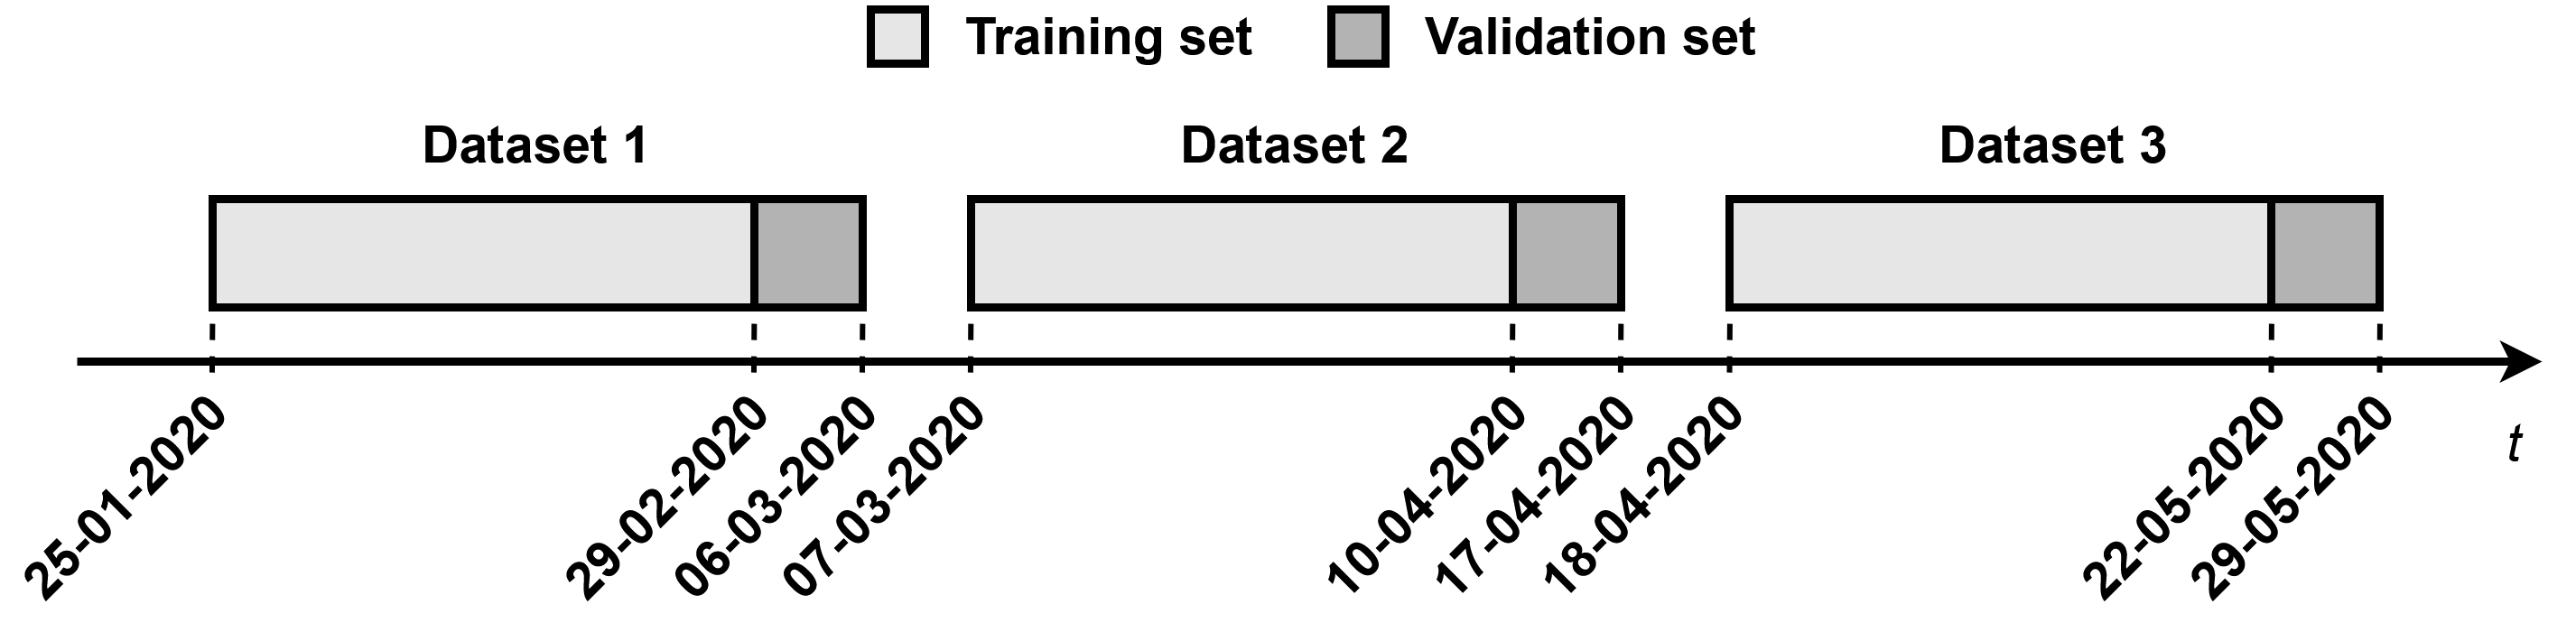
\includegraphics[width=1\textwidth]{Images/hyptun.png}
    \caption{Datasets used for expanding window cross-validation.}
    \label{hyptun}
    \end{center}
\end{figure}

The process of tuning hyperparameters is a long and time consuming process. Although the meaning of each hyperparameter and what it represents in the context of the layer is known, there is no rule dictating which hyperparamters are best for each case. It is an experimental process in which the models must be trained, and validated. The results obtained in the validation data are then compared for different hyperparameter combinations. The combination that presents the best results for each model, must be the one selected. To speed up this process, a script \cite{} was created, responsible for training and validating multiple combinations of hyperparameters for each of the proposed models. In total, about 84 different combinations were tested in each of the four blocks. Based on the results obtained in each block for each of the 84 combinations, the ideal hyperparameter combination for each of the six proposed models is defined, being the one that, on average, presents a lower error value in the four cases. In Appendix XXXX, one can find the tables with the validation errors registered for each of the four blocks.

As explained earlier, exhaustive grid-search was then used to test various combinations of hyperparameters for each of the models. In the layers \ac{GRU} and \ac{LSTM}, the number of units of each layer was consecutively changed.
The number of units is a positive integer that represents the dimensionality of the output space of the layer. This hyperparameter must be tuned in to find a value for which the system performs well. However, the increase of this value represents an increase in the complexity of the model, which makes it slower. Regarding the \ac{1D CNN} layers, the hyperparameters that were tested were the number of filters - An integer that represents dimensionality of the output space (i.e. the number of output filters in the convolution), the kernel\_size - An integer specifying the length of the 1D convolution window used. In the Max pooling layer, a pool\_size was fixed to 2 units, which means that only the highest value every 2 values is taken into account, as explained in the section \ref{chap3:subsubsec:1dcnn}. In order to avoid overfitting, dropout layers with $p=0.2$ were also used.

For each of the four blocks defined in the expanding window cross-validation process, the architectures were trained and validated. The hyperarameters already mentioned were progressively optimized in the four blocks, for each model. The Table \ref{tab:characteristics} details the number of inputs, hidden layers and hidden nodes of each model. 


% Table generated by Excel2LaTeX from sheet 'Sheet6'
\begin{table}[htbp]
  \centering
  \caption{Hyperparameters of the selected models.}
    \begin{tabular}{r|cccc}
    \multicolumn{1}{c|}{\multirow{2}[1]{*}{\textbf{Model}}} & \multicolumn{2}{c}{\textbf{Vanilla}} &   &  \\
      & GRU & LSTM &   &  \\
\cmidrule{1-3}    \# inputs & 13 & 13 &   &  \\
    \# hidden layers & 1 & 1 &   &  \\
    \# hidden nodes & 128 & 64 &   &  \\
    \midrule
    \multicolumn{1}{c|}{\multirow{2}[2]{*}{\textbf{Model}}} & \multicolumn{4}{c}{\textbf{Encoder-Decoder}} \\
      & GRU-GRU & LSTM-LSTM & 1D CNN-GRU & 1D CNN-LSTM \\
    \midrule
    \# inputs & 13 & 13 & 13 & 13 \\
    \# encoder nodes & 16 & 256 & 16 & 16 \\
    \# decoder nodes & 16 & 256 & 8 & 64 \\
    \end{tabular}%
  \label{tab:characteristics}%
\end{table}%





In Table \ref{valres}, the reader may consult the results of the expanding window cross-validation process, which consists of an average of the errors presented in blocks 1, 2, 3 and 4.

% Table generated by Excel2LaTeX from sheet 'Tabel Creation'
\begin{table}[htbp]
  \centering
  \caption{Add caption}
    \begin{tabular}{r|cc|cccc}
    \multicolumn{1}{c|}{\multirow{2}[1]{*}{\textbf{Model}}} & \multicolumn{2}{c|}{\textbf{Vanilla}} & \multicolumn{4}{c}{\textbf{Encoder-Decoder}} \\
      & GRU & LSTM & GRU-GRU & LSTM-LSTM & 1D CNN-GRU & 1D CNN-LSTM \\
    \midrule
    \textbf{Validation (t+5)} &   &   &   &   &   &  \\
    RMSE (E-02) & 2.895 & 3.001 & 2.661 & 2.783 & 2.756 & 2.739 \\
    MSE(E-03) & 0.854 & 0.917 & 0.714 & 0.780 & 0.762 & 0.753 \\
    MAE (E-02) & 2.055 & 2.146 & 1.925 & 2.101 & 2.051 & 2.040 \\
    \textbf{Validation (t+10)} &   &   &   &   &   &  \\
    RMSE (E-02) & 3.316 & 3.498 & 3.076 & 3.141 & 3.139 & 3.145 \\
    MSE(E-03) & 1.114 & 1.246 & 0.951 & 0.989 & 0.987 & 0.992 \\
    MAE (E-02) & 2.384 & 2.502 & 2.244 & 2.360 & 2.329 & 2.353 \\
    \textbf{Validation (t+15)} &   &   &   &   &   &  \\
    RMSE (E-02) & 3.599 & 3.705 & 3.354 & 3.466 & 3.438 & 3.444 \\
    MSE(E-03) & 1.317 & 1.386 & 1.130 & 1.204 & 1.184 & 1.189 \\
    MAE (E-02) & 2.585 & 2.709 & 2.454 & 2.609 & 2.546 & 2.578 \\
    \midrule
    \textbf{Total Validation} &   &   &   &   &   &  \\
    RMSE (E-02) & 3.270 & 3.402 & 3.031 & 3.130 & 3.111 & 3.109 \\
    MSE(E-03) & 1.095 & 1.183 & 0.932 & 0.991 & 0.978 & 0.978 \\
    MAE (E-02) & 2.342 & 2.453 & 2.208 & 2.357 & 2.309 & 2.324 \\
    \end{tabular}%
  \label{valres}%
\end{table}%





The Table presents the validation \ac{MSE}, \ac{RMSE} and \ac{MAE} for each one of the models, both for the individual forecast for power available in 5, 10 and 15 minutes.



(COMENTÁRIOS AOS DADOS)

\section{Stage 2 - Results}\label{chap3:section:stage_2}

In the previous step, the six models that presented the best performance for the defined scenarios were defined. In this step, the six models are trained again in all available training data, which consists of training the models in the whole block 4 and testing their performance in the test data. In Figure \ref{test} the reader can find a graphic representation of this process.

\begin{figure}[h!]
    \centering
    \begin{center}
    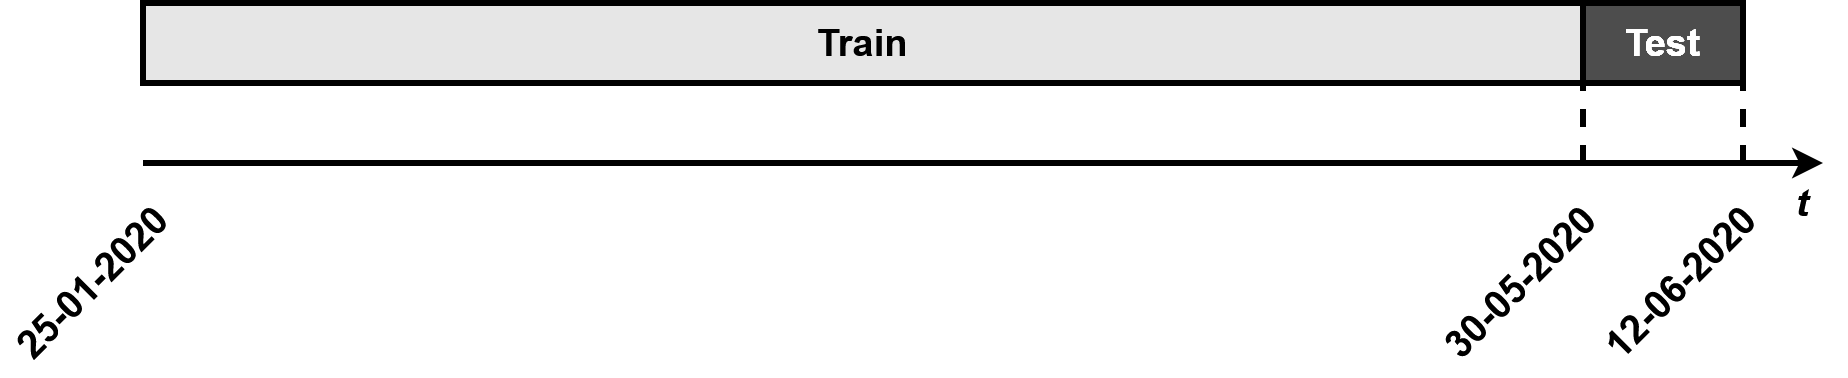
\includegraphics[width=1\textwidth]{Images/test2.png}
    \caption{Dataset used for testing the final models.}
    \label{test}
    \end{center}
\end{figure}

\section{Stage 3 - Confidence intervals}\label{chap3:section:stage_3}

It is true that the main goal is to set a value for the available power at 5, 10 and 15 minutes, but it would be interesting to set a maximum and a minimum value for each of these three forecasts. In other words, it would be important to be able to project a confidence interval of the forecasts carried out. 

In order to project the confidence interval of a forecast from a set of points $x(t, ..., N)$, multiple sets of values are needed for this interval, that is, based on the same input data, the model would have to be able to generate several forecast values for this instant, but this does not happen. As we know, \ac{ANNs}, after the training process in which the weights are defined, become deterministic functions, which means that for the same input, the same predicted output will always be produced, regardless of the number of times the algorithm runs. We are then faced with a limitation, the impossibility of obtaining several values for the same instant, so that a confidence interval of the forecast can be computed.

In 2017, Zhu proposed a technique to solve this problem \cite{uber}. The principle is to adapt the predictive model so that it can return multiple (different) predictions by applying dropout in the forecast process. As discussed in section \ref{chap3:subsubsec:regularization_techniques}, one of the most common techniques to avoid overfitting is the use of dropout layers. Usually, these layers are active in the training process, in order to introduce some error in the model to prevent it from overadapting to the data provided. But in the testing phase, these layers are disabled. The application of dropout "turns off" a randomly chosen fraction of the units of the model. Applying dropout in the testing process would imply that the model ceases to be deterministic, that is, for the same input, different outputs are generated each time forecasts are made. 
This principle is also known as Mote Carlo \cite{uber2} dropout, which dictates that the uncertainty of the model can be estimated by sample variance of the forecasts of the adapted model in some repetitions. For example, if for each input sequence, 100 distinct output sequences are predicted, assuming the dropout is maintained, all 100 sequences are different. By averaging the 100 sequences, one obtains an average forecast of the model, which can be assumed to be the actual result of the model forecast, that can be called MC Dropout Forecast. On the other hand, since for each instant you have 100 different values, the standard deviation of the 100 values can then be used to calculate the confidence interval of each of the values and, ultimately, the complete sequence. Assuming that the forecasts have a normal distribution $N(\mu, \sigma^2)$, with a mean $\mu$ and a standard deviation $\sigma$, it is then possible to determine the confidence intervals given by: 

\begin{equation}
    [\hat{y}^* - z_{\frac{\alpha}{2}}\mu,\ \hat{y}^* + z_{\frac{\alpha}{2}}\mu], 
\end{equation}

where $\hat{y}^* = \frac{1}{B}\sum_{b=1}^B\hat{y_b}$ and $\mu = \sqrt{\frac{1}{B}\sum_{b=1}^B(\hat{y_b} -\hat{y}^*)^2}$. In order to to compute the 95\% confidence interval, for example, the parameters should be $\alpha=0.05$ and $z_{\frac{\alpha}{2}}= 1.92$ . 

Another consideration that should be made is the selection of the parameter $p$ in the MC dropout. If the MC dropout is too large, the forecasts generated will be quite sparse, which in turn implies that the confidence intervals created will be too large. On the other hand, if the MC dropout is too small, the forecasts made will be too similar to each other, which results in very small confidence intervals. When $p$ value is ideal, there is an almost perfect correspondence between the confidence interval and the values obtained. For the problem in question, the parameter $p$ of the MC dropout was tested for various values, and it was concluded that a good value would again be $p = 0.2$.

In Figure XXX we can see the result of applying the Monte Carlo dropout method.

\begin{figure}[h!]
    \centering
    \begin{center}
    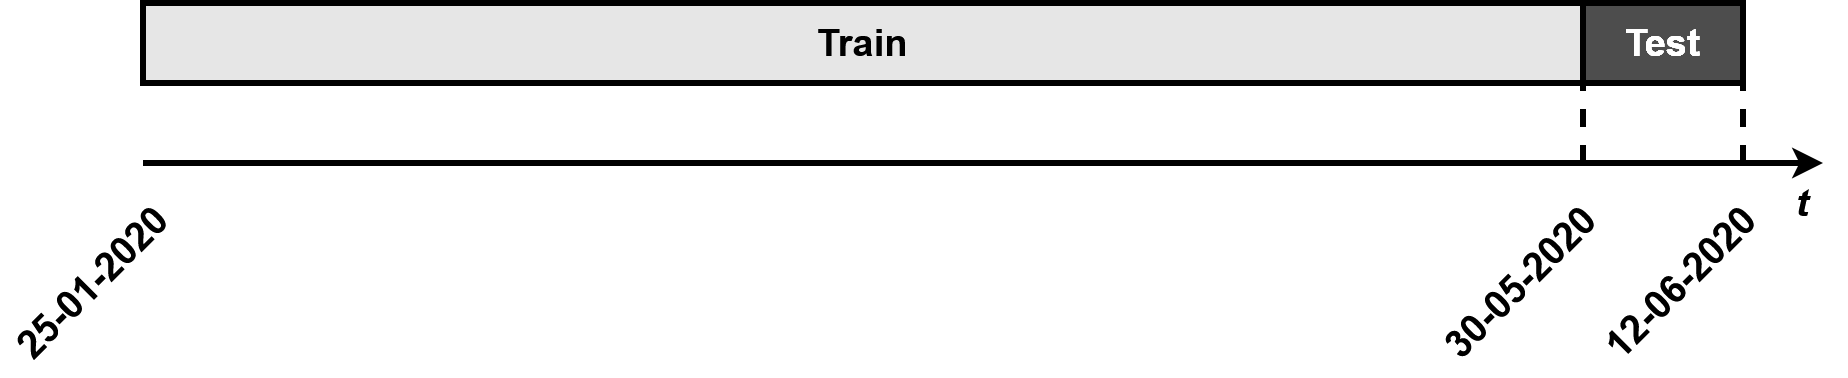
\includegraphics[width=1\textwidth]{Images/test2.png}
    \caption{Dataset used for testing the final models.}
    \label{test}
    \end{center}
\end{figure}


Another issue to consider is that in the standard model, which applies dropout only in the training process, only one forecast sequence is produced, which can be called Standard Dropout Forecast. In the case where a dropout is applied in the training process and MC Dropout in the test process, a set of $N$ sequences, defined by the user, is obtained. The forecast produced in this second case is an average of the $N$ sequences produced, which can be called MC Dropout Forecast. It would be intuitive to assume that MC Dropout Forecast, since it is computed based on a set of different $N$ tests, presents a more robust estimate for the predicted values. However, the experiment was performed, where each of the 6 finalist architectures tested, for the case where it features Standard Dropout, and for the case where it features MC Dropout. The results obtained can be confirmed in Table xxx. 

TABELA


COMMENTS.

Although the results obtained for models with MC Dropout present a lower \ac{RMSE} value, it should be remembered that the forecasts resulting from the application of Standard Dropout are generated with a single iteration of the forecast process, while the models that apply MC Dropout result from N iterations. The more iterations carried out, the more accurate the stipulated interval will be, however the forecasting process will also take longer. It is then necessary to balance the value of $N$ with the time that $N$ iterations take to be processed. In very short-term forecasting models, as is the case, this factor is preponderant since the granularity of the data is very high and the forecasts should be immediate. It is also a factor that is directly linked to the available computing capacity.


